\documentclass[11pt,a4paper]{article}
\usepackage[margin=2.6cm]{geometry}
\usepackage{amsmath,amssymb}
\usepackage{graphicx}
\usepackage{booktabs}
\usepackage[hidelinks]{hyperref}
\usepackage{xcolor}
\usepackage{caption}
\captionsetup{font=small,labelfont=bf}
\setlength{\parskip}{4pt}
\setlength{\parindent}{0pt}

\newcommand{\vrel}{v_{\mathrm{rel}}}
\newcommand{\vorb}{v_{\mathrm{orb}}}
\newcommand{\Rint}{R_{\mathrm{int}}}
\newcommand{\Rest}{R_{\mathrm{est}}}
\newcommand{\Rbar}{\bar{R}}
\newcommand{\nbar}{\bar{n}}
\newcommand{\Eacc}{E_{\mathrm{acc}}}
\newcommand{\ieff}{i_{\mathrm{eff}}}

\title{Collision Risk in LEO Mega-Constellations:\\
from the Kinetic-Gas Model to the Keplerian Model\\
\large Analytic treatment, convergence study, and Monte Carlo validation}
\author{Prepared by Claude Fable 5 (Anthropic)\\
under the supervision of Alessandro Golkar\\
Technical University of Munich \\ \texttt{golkar@tum.de}}
\date{June 2026}

\begin{document}
\maketitle

\begin{center}
\fbox{\parbox{0.92\textwidth}{\small
\textbf{Notice.} This model and report were generated by Claude Fable 5 (Anthropic),
an AI system, under the supervision of Alessandro Golkar, and are currently
undergoing verification. Do not trust the model results unless manually verified.
An interactive companion implementing all models in this report is available at
\texttt{https://megaconstellations.golkar.ai}; bugs, comments and feedback are
welcome at \texttt{golkar@tum.de}.\\[2pt]
\copyright~2026 Alessandro Golkar, Technical University of Munich.}}
\end{center}

\begin{abstract}
We develop and compare two models of the collision rate in a mega-constellation of
$N = 80{,}000$ compute satellites with $120\,\mathrm{m}^2$ radiators occupying the
500--800~km altitude band: the kinetic-gas baseline (Kessler particle-in-a-box with
isotropic velocities) and a Keplerian kinetic model built from the orbit-element
distributions. The central hypothesis is confirmed in a precise form: for large $N$
with randomized RAAN and mean anomaly, the Keplerian collision statistics converge
exactly to a kinetic theory of the form $\mathrm{rate} = n\,\sigma\,\vrel$, but with a
structured, anisotropic density field $n(r,\beta)$ and a discrete, latitude-dependent
relative-velocity spectrum; convergence is \emph{not} to isotropic Brownian motion.
For the reference scenario the Keplerian model gives $1941$ collisions per year against
the baseline's $2608$, a ratio of $0.744$ that decomposes into a spatial anisotropy
enhancement $F_{\mathrm{sp}} \approx 1.22$ and a velocity-structure reduction
$F_{\mathrm{vel}} \approx 0.61$. Direct conjunction counting with exact two-body
propagation reproduces the analytic rate to $0.3\% \pm 3.2\%$. Neither model admits a
geometric solution: the shell thickness required to reach one collision per year exceeds
the geostationary altitude. The collision burden must be managed by active avoidance,
cross-section control, and population control, and the constellation sits far beyond a
simple Kessler-cascade boundary unless post-collision debris generation is suppressed.
An extended systems model couples the collision engine to thermal, power, and
attitude-control sizing and to the external debris environment. Its principal additions:
the photovoltaic array, not the radiator, dominates the deployed area, multiplying the
natural rate by 7 when counted in the cross-section; the thermally preferred
Sun-synchronous architecture pays a 38.5\% collision premium; and lethal non-trackable
debris adds a loss channel of order $10^3$ per fleet-year that no avoidance reliability
can reduce.
\end{abstract}

\section{Background and context}

The statistical treatment of orbital collisions has a fifty-year lineage. \"Opik (1951)
derived the intrinsic collision probability between two bodies on independent orbits for
planetary applications; Wetherill (1967) generalized the geometry for asteroid
populations. Kessler and Cour-Palais (1978) imported the kinetic theory of gases into the
artificial-satellite problem: treat the population as a dilute gas with number density
$n$, collision cross-section $\sigma$, and characteristic relative speed $\vrel$, so that
each object suffers collisions at rate $\nu = n \sigma \vrel$. That paper predicted the
debris-belt feedback now known as the Kessler syndrome. Kessler (1981) then replaced the
uniform-gas assumption with the time-averaged spatial density of actual inclined orbits,
which concentrates objects near their turning latitudes. Modern debris-evolution codes
descend from both ideas: NASA's LEGEND model (Liou et al.\ 2004) propagates objects
deterministically and applies kinetic theory locally in sampled volume cells (the
``Cube'' method), which is the operational bridge between deterministic dynamics and
gas-like statistics.

Two developments make a re-examination timely. First, mega-constellations have moved the
relevant population from thousands of uncontrolled debris objects to tens of thousands of
\emph{controlled} satellites with similar orbits, where the isotropic-gas closure is least
justified. Second, proposals for orbital data centers (tens of thousands of satellites
whose computing payloads require radiators of order $100\,\mathrm{m}^2$) couple a thermal
design variable directly to the collision cross-section: heat rejection wants area, and
collision probability grows with it. Public filings made in 2026 for constellations of up
to 88{,}000 compute satellites match the scale studied here.

This report does three things. It reproduces the kinetic-gas baseline for the reference
scenario as an anchored benchmark. It constructs the full Keplerian kinetic model, with
the spatial density field and the admissible-velocity structure derived from the orbit
elements, and states precisely in what sense and under what conditions the Keplerian
statistics converge to the kinetic form (they do, but to an anisotropic, structured
kinetic theory, and not to an isotropic gas). And it validates the analytic rate against
direct conjunction counting with exact two-body propagation, before drawing the design
consequences for radiator sizing, avoidance load, and the cascade boundary.

\section{Problem statement and notation}

A constellation of $N$ satellites occupies the spherical shell between geocentric radii
$\Rint = 6871$~km and $\Rest = 7171$~km (altitudes 500 and 800~km, $R_E = 6371$~km).
Each satellite carries a radiator of area $A = 120\,\mathrm{m}^2$ (reference: an
``AI1''-class orbital compute satellite), which dominates its physical extent. The
exposure window is $T = 1\,\mathrm{yr} = 3.156\times10^{7}\,\mathrm{s}$. All
parameters below are inputs of the computational engine
(\texttt{collision\_models.py}); the values quoted are the reference case.

\begin{table}[h]\centering\small
\begin{tabular}{llll}
\toprule
Symbol & Meaning & Reference value & Status \\
\midrule
$N$ & satellites & $80{,}000$ & input \\
$A$ & radiator area & $120\,\mathrm{m}^2$ & input \\
$\sigma$ & collision cross-section & $4A = 480\,\mathrm{m}^2$ & input (shape factor $\times A$) \\
$\Rint,\ \Rest$ & shell radii & 6871, 7171 km & input \\
$\{(i_k, w_k)\}$ & inclination mix & $43^\circ/53^\circ/70^\circ/97.6^\circ$, $w = 0.2/0.4/0.2/0.2$ & input \\
$\delta i$ & inclination dispersion & $\pm0.5^\circ$ uniform & input \\
$f_{\mathrm{fail}}$ & avoidance failure fraction & 1 (natural rate) & input \\
$V$ & shell volume & $1.859\times10^{20}\,\mathrm{m}^3$ & derived \\
$\nbar$ & mean density $N/V$ & $4.30\times10^{-16}\,\mathrm{m}^{-3}$ & derived \\
$\vorb$ & circular speed at $\Rbar = 7021$ km & $7535\,\mathrm{m/s}$ & derived \\
$\vrel^{\mathrm{iso}}$ & baseline relative speed & $10^4\,\mathrm{m/s}$ & input \\
\bottomrule
\end{tabular}
\caption{Inputs and derived quantities. The engine keeps the two strictly separate.}
\end{table}

The cross-section convention follows the enveloping-sphere argument: with equivalent
radius $r = \sqrt{A/\pi}$, two centers collide within $2r$, hence $\sigma = \pi (2r)^2
= 4A$. For a flat plate in random attitude the orientation-averaged projected area is
about half the face area and the enveloping sphere is mostly empty, so the physical
cross-section lies a factor 2--4 lower. We keep $\sigma = 4A$ as the nominal value and
carry the shape factor as an explicit parameter; every rate below scales linearly
in~$\sigma$.

\section{Model 1: the kinetic-gas baseline}

\subsection{Assumptions and rate}

Satellites are treated as molecules of a dilute gas in isotropic random motion inside
the shell (Kessler 1978). The three assumptions are: spatially uniform density
$\nbar = N/V$; a single scalar relative speed $\vrel = \sqrt{2}\,\bar v \approx
10$~km/s; and statistical independence of all positions (dilute, uncorrelated gas).
The per-satellite collision frequency and fleet-wide expectation are
\begin{equation}
\nu \;=\; \nbar\,\sigma\,\vrel, \qquad
P_1(T) = 1 - e^{-\nu T} \approx \nu T, \qquad
E[\mathrm{collisions}] \;=\; \tfrac12\,N\,\nu\,T \;=\; \frac{N^2 \sigma \vrel T}{2V},
\end{equation}
where the factor $\tfrac12$ avoids double-counting pairs.
Dimensional check: $[\mathrm{m}^{-3}][\mathrm{m}^2][\mathrm{m\,s}^{-1}] =
\mathrm{s}^{-1}$, as required.

\subsection{Reference results (anchor)}

\begin{table}[h]\centering\small
\begin{tabular}{lll}
\toprule
Quantity & Value & Order check \\
\midrule
$V$ & $1.859\times10^{20}\,\mathrm{m}^3$ & $4\pi \Rbar^2 \Delta r = 1.86\times10^{20}$ (thin shell, $-0.1\%$) \\
$\nbar$ & $4.30\times10^{-16}\,\mathrm{m}^{-3}$ & one satellite per $2.3\times10^{6}\,\mathrm{km}^3$ \\
$\nu$ & $2.07\times10^{-9}\,\mathrm{s}^{-1} = 0.0652\,\mathrm{yr}^{-1}$ & $4.3\times10^{-16}\cdot480\cdot10^4$ \\
$P_1$ & $6.3\%$ per year & $\approx \nu T$, Poisson valid since $\nu T \ll 1$ \\
$E$ & $\mathbf{2608}$ per year & anchor $\approx 2600$ reproduced \\
$\lambda$ & $3.4\times10^{9}$ km & see correction below \\
\bottomrule
\end{tabular}
\caption{Kinetic baseline, reference case. Realistic band 600--2600 per year
depending on the cross-section treatment (shape factor 1--4).}
\end{table}

\textbf{A correction to the baseline record.} The mean free path is
$\lambda = (\sqrt{2}\,\nbar\,\sigma)^{-1} = 3.4\times10^{12}\,\mathrm{m}
= 3.4\times10^{9}$~km, not $9\times10^{10}$~km as previously recorded; the equivalent
kinematic estimate $\vrel/\nu = 4.8\times10^{9}$~km agrees in order. The conclusion is
unchanged and in fact strengthened only in bookkeeping: $\lambda$ exceeds the shell
thickness by a factor $\sim 10^{7}$, the gas is extremely dilute, and Poisson
statistics are valid.

Gravitational focusing is negligible: the enhancement factor is
$1 + (v_{\mathrm{esc}}/\vrel)^2$ with $v_{\mathrm{esc}}$ the two-body escape speed at
contact, below $\mathrm{mm/s}$ for tonne-class satellites at tens of meters, giving
corrections of order $10^{-14}$.

\subsection{Inversion: the geometric dead end}

Requiring $E \le \Eacc$ and inverting for the shell volume gives
\begin{equation}
V_{\mathrm{req}} = \frac{N^2 \sigma \vrel T}{2\Eacc}, \qquad
\Delta r \approx \frac{N^2 \sigma \vrel T}{8\pi \Rbar^2 \Eacc}
\;\;\Rightarrow\;\;
\Delta r\,[\mathrm{km}] \approx \frac{7.8\times10^{5}}{\Eacc},
\end{equation}
the thin-shell form being valid only for $\Delta r \ll \Rbar$, i.e.\ $\Eacc \gg 100$.
Solving the exact cubic with $\Rint$ fixed: $\Eacc = 100$ requires $\Delta r = 4543$~km;
$\Eacc = 10$ requires $16{,}000$~km; $\Eacc = 1$ requires $41{,}900$~km, beyond
geostationary altitude (Figure~\ref{fig:inversion}). No physically sensible LEO shell
geometry reaches an acceptable threshold. The kinetic model is therefore a
\emph{diagnostic} instrument quantifying the collision-avoidance burden, not a design
tool for shell geometry: the real levers are active control, cross-section, and
population.

\begin{figure}[h]\centering
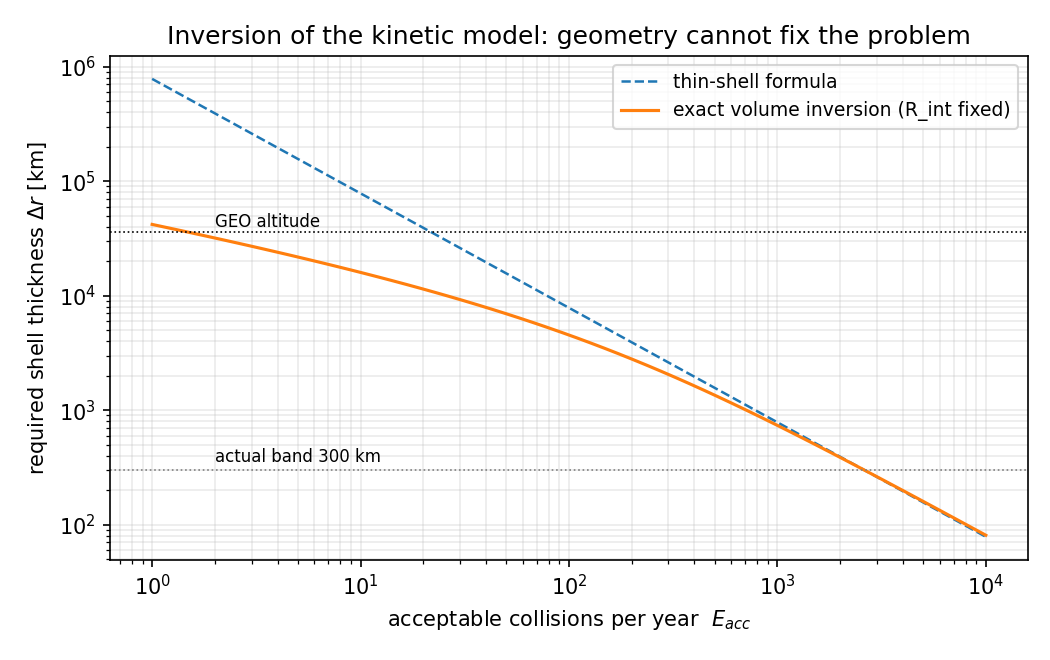
\includegraphics[width=0.72\textwidth]{figures/fig6_shell_inversion.png}
\caption{Shell thickness required to bring the natural collision rate below
$\Eacc$. The dashed line is the thin-shell formula, the solid line the exact volume
inversion. Both cross the GEO altitude before reaching $\Eacc \sim 1$.}
\label{fig:inversion}
\end{figure}

\section{Model 2: the Keplerian kinetic model}

The baseline's random-walk picture is dynamically wrong: satellites move on
deterministic near-circular orbits, and at any point in space only the velocity
vectors compatible with an orbit of that energy through that point are admissible.
We now build the collision rate from the orbit-element distributions, for circular
orbits with inclination mix $\{(i_k, w_k)\}$, uniform RAAN, uniform phase, and a
radial distribution $g(r)$ across the band.

\subsection{Spatial density field}

A single circular orbit of inclination $i$ spends, per unit latitude, the time
fraction
\begin{equation}
p(\beta\,|\,i) \;=\; \frac{1}{\pi}\,
\frac{\cos\beta}{\sqrt{\sin^2 \ieff - \sin^2\beta}},
\qquad |\beta| < \ieff \equiv \min(i, \pi - i),
\label{eq:latpdf}
\end{equation}
which integrates to unity and has the well-known integrable pile-up at the turning
latitudes $\beta = \pm\ieff$ (Kessler 1981). With RAAN uniform the density is
azimuthally uniform, and dividing by the area of the latitude band gives the
number density of population $k$,
\begin{equation}
n_k(r, \beta) \;=\; N_k\, g(r)\, \frac{p(\beta\,|\,i_k)}{2\pi r^2 \cos\beta},
\qquad \int n_k \, \mathrm{d}V = N_k .
\label{eq:density}
\end{equation}
For the uniform-volume profile, $g(r) = 3r^2/(\Rest^3 - \Rint^3)$. The resulting
field (Figure~\ref{fig:density}) concentrates at the cap latitudes of each
inclination population, peaking at $4.3\times$ the mean density near $\pm 53^\circ$
for the reference mix.

\begin{figure}[h]\centering
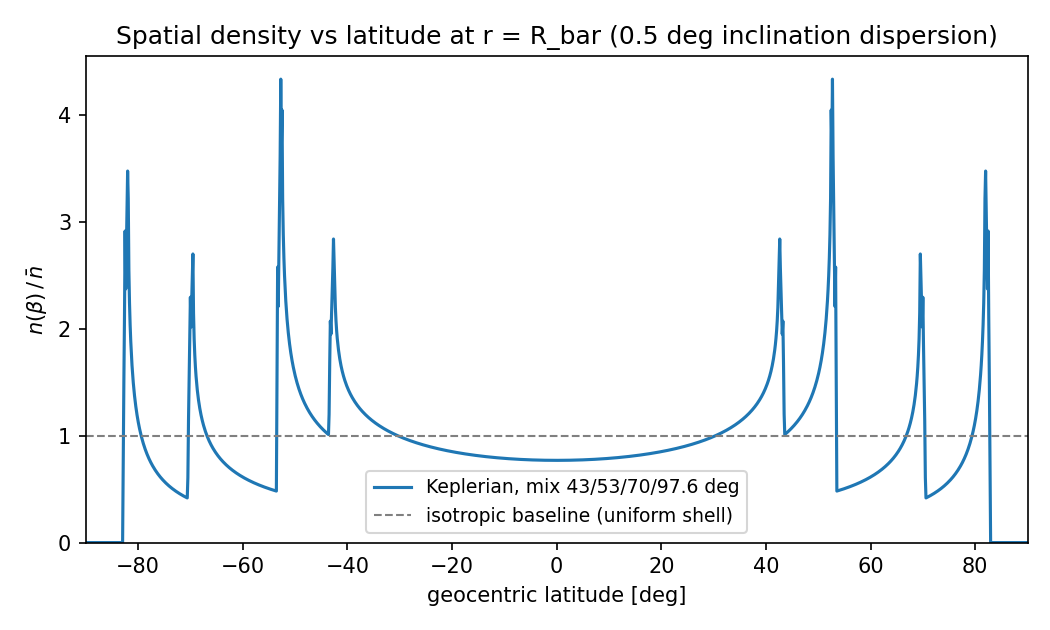
\includegraphics[width=0.72\textwidth]{figures/fig1_density_latitude.png}
\caption{Keplerian density versus latitude at $r = \Rbar$ for the reference mix,
normalized to the uniform-shell value. Each population piles up at its cap
latitude; the $97.6^\circ$ sun-synchronous population caps at $82.4^\circ$.}
\label{fig:density}
\end{figure}

\subsection{Local velocity structure}

At latitude $\beta$, a circular orbit of inclination $i$ crosses with heading
(angle from local East)
\begin{equation}
\cos A = \frac{\cos i}{\cos\beta}, \qquad
\sin A = \frac{\sqrt{\sin^2 \ieff - \sin^2 \beta}}{\cos\beta},
\qquad A \in [0, \pi],
\end{equation}
the ascending pass taking $+A$ and the descending pass $-A$, each half the time;
retrograde orbits ($\cos i < 0$) give $A > \pi/2$. Two satellites from populations
$j$ and $k$ meeting at $(r,\beta)$ therefore have exactly two admissible
relative-speed branches,
\begin{equation}
\vrel = 2\vorb \sin\frac{\theta}{2}, \qquad
\theta \in \{\, |A_j - A_k| \ \text{(same sense)},\;\; A_j + A_k \ \text{(opposite sense)} \,\},
\label{eq:vrelbranches}
\end{equation}
each carrying probability $\tfrac12$, so that
$\langle \vrel \rangle_{jk}(\beta) = \vorb\,[\sin(|A_j - A_k|/2) + \sin((A_j+A_k)/2)]$.
This replaces the Maxwellian: the spectrum is discrete at each latitude, governed
entirely by the inclination distribution. Two consistency properties are built in.
For $j = k$ the same-sense branch has $\theta = 0$: two co-altitude satellites of the
same inclination passing the same point in the same sense are coplanar and co-orbital
and never collide. And at the cap latitude $\beta \to \ieff$ all headings become
East-West, $\vrel \to 0$: exactly where the density diverges, the velocities become
parallel.

\subsection{The rate integral}

With randomized RAAN and phase the positions of distinct satellites are statistically
independent, so the pair density factorizes exactly and the fleet-wide rate is
\begin{equation}
R \;=\; \frac{1}{2}\sigma \int \sum_{j,k} n_j n_k \,\langle\vrel\rangle_{jk}\,\mathrm{d}V
\;=\; \frac{1}{2}\,\sigma\, I_r \sum_{j,k} N_j N_k\, J_{jk},
\label{eq:rate}
\end{equation}
which separates into a radial factor and latitude integrals
\begin{equation}
I_r = \int \frac{g(r)^2}{2\pi r^2}\,\mathrm{d}r, \qquad
J_{jk} = \int_{-\beta_{\max}}^{\beta_{\max}}
\frac{p(\beta|i_j)\, p(\beta|i_k)}{\cos\beta}\,
\langle\vrel\rangle_{jk}(\beta)\,\mathrm{d}\beta ,
\label{eq:Jjk}
\end{equation}
with $\beta_{\max} = \min(i_{\mathrm{eff},j}, i_{\mathrm{eff},k})$ and $\vorb$ evaluated at $\Rbar$ (its
variation across the band is below 2\%, declared as an approximation). For the
uniform-volume profile $I_r = 2/V$ exactly, and if one artificially sets
$n_k$ uniform and $\langle\vrel\rangle$ constant, Eq.~\eqref{eq:rate} collapses to
the baseline $N^2 \sigma \vrel/2V$: the kinetic model is the structureless limit of
Eq.~\eqref{eq:rate}. The substitution $\sin\beta = \sin\beta_{\max}\sin\phi$ removes
the endpoint singularity and the integrals are evaluated with Gauss-Legendre
quadrature; results are converged to four digits at 400 nodes.

\subsection{The cap singularity and the role of inclination dispersion}
\label{sec:dispersion}

For a population with a mathematically exact single inclination, the density-squared
integral $\int n^2\,\mathrm{d}V$ diverges logarithmically at the caps, since
$n \sim (\ieff - \beta)^{-1/2}$. The \emph{rate} remains finite because
$\langle\vrel\rangle$ vanishes there at the same order, so the integrand of
Eq.~\eqref{eq:Jjk} behaves as $(\ieff-\beta)^{-1/2}$, which is integrable. The
physical regularization is the finite inclination spread $\delta i$ of any real
population. The consequence, verified numerically, is a clean and slightly subtle
statement:
the total rate is insensitive to $\delta i$ (1941.4, 1941.3, 1941.9 collisions/yr at
$\delta i = 0.1^\circ, 0.5^\circ, 2^\circ$), while the decomposition into a spatial
factor and a velocity factor depends on $\delta i$ logarithmically
($F_{\mathrm{sp}} = 1.33, 1.22, 1.13$ at the same three spreads). Only the product
$F_{\mathrm{sp}} F_{\mathrm{vel}}$, i.e.\ the rate itself, is a robust observable; the
split is reported at the reference dispersion $\delta i = 0.5^\circ$.

\section{The convergence hypothesis: confirmed, with precision}
\label{sec:convergence}

\textbf{Statement.} For $N \to \infty$ with randomized elements, Keplerian collision
statistics converge to a kinetic theory of the form
$\mathrm{rate} = n\,\sigma\,\vrel$, with $n$ the anisotropic field
\eqref{eq:density} and $\vrel$ the structured spectrum \eqref{eq:vrelbranches}.
Convergence is \emph{not} to the isotropic Brownian gas: the Maxwellian assumption is
replaced by the orbit-admissibility constraint, and the uniform density by the
latitude-structured field. The hypothesis as posed is therefore confirmed in its
refined form: Kessler's functional form survives; the isotropic closure does not.

\textbf{Criterion.} Three conditions, each quantitative, govern the convergence.

\emph{(i) Ensemble factorization (exact).} With RAAN and mean anomaly independently
uniform, the two-point density factorizes exactly at any $N \ge 2$:
Eq.~\eqref{eq:rate} is the exact ensemble mean, not a large-$N$ limit. Differential
$J_2$ nodal precession across the band supplies the physical randomization of RAAN
over months even from an initially organized deployment, and phase mixing randomizes
anomalies within days.

\emph{(ii) Self-averaging of a specific draw.} A particular constellation realizes one
draw of the pairwise rate sum. Its relative fluctuation around the ensemble mean
scales as $c/\sqrt{N_{\mathrm{pairs}}^{\mathrm{eff}}}$, where
$N_{\mathrm{pairs}}^{\mathrm{eff}}$ is the number of pairs that can actually meet
(radial shells must overlap within the collision radius) and $c$ is the coefficient
of variation of pair rates ($c \sim 10$ for this mix, measured from seed-to-seed
scatter in the Monte Carlo runs). This exposes a hidden requirement: \emph{radial}
randomization. For strictly circular orbits spread over a 300~km band, only pairs
within $\sim$12~m in radius can collide; eccentricity dispersion of order
$e \sim 10^{-3}$ (radial excursions of $\pm 7$~km) raises
$N_{\mathrm{pairs}}^{\mathrm{eff}}$ to $\sim 10^{8}$ at $N = 80{,}000$ and makes the
fluctuation negligible. At small $N$ or perfectly coordinated radial station-keeping,
a specific constellation can sit tens of percent away from the kinetic mean.

\emph{(iii) Poisson time statistics.} On time scales long compared to the orbital and
synodic periods, encounter events for a given satellite are well modeled as a Poisson
process with the rate of Eq.~\eqref{eq:rate}, since $\nu T \ll 1$ and successive
encounters involve effectively independent partners.

\textbf{The isotropic limit as an internal test.} If inclinations are drawn with
$\cos i \sim U(-1,1)$, orbit normals are isotropic, the density field becomes exactly
uniform on the sphere, and headings become uniform in the local tangent plane. The
model then must reduce to a kinetic gas, but with the tangent-plane average
$\langle \vrel\rangle = \frac{4}{\pi}\vorb = 9594$~m/s, which differs from the 3-D
isotropic value $\frac{4}{3}\vorb = 10{,}046$~m/s: even a fully randomized satellite
population is not a 3-D gas, because all speeds are equal and all velocities are
horizontal. The engine reproduces this limit: ratio to baseline $0.9565 \pm 0.0070$
measured against $4\vorb/\pi/10^4 = 0.9594$ predicted, and $F_{\mathrm{sp}} = 0.992$.
This also explains quantitatively why the canonical 10~km/s baseline lands close to
the truth despite the wrong velocity distribution.

\section{Results for the reference scenario}

\subsection{Rates and correction factors}

\begin{table}[h]\centering\small
\begin{tabular}{lcc}
\toprule
 & Kinetic baseline & Keplerian model \\
\midrule
$E$[collisions], natural, per year & 2608 & \textbf{1941} \\
mean per-satellite $\nu$ [yr$^{-1}$] & 0.0652 & 0.0485 \\
per-satellite $P_1$ per year & 6.3\% & 4.7\% (mean) \\
rate-effective $\langle\vrel\rangle$ & $10$ km/s (assumed) & $6.09$ km/s (derived) \\
mean impact speed (collision-weighted) & 10 km/s & 10.2 km/s \\
\bottomrule
\end{tabular}
\caption{Reference scenario, natural rates ($f_{\mathrm{fail}} = 1$), $\sigma = 4A$.}
\label{tab:main}
\end{table}

The Keplerian-to-baseline ratio is
\begin{equation}
\frac{R_{\mathrm{kep}}}{R_{\mathrm{kin}}} = 0.744
\;=\; \underbrace{F_{\mathrm{sp}}}_{1.22}\,\times\,\underbrace{F_{\mathrm{vel}}}_{0.61},
\end{equation}
at $\delta i = 0.5^\circ$ (Section~\ref{sec:dispersion}). The two corrections pull in
opposite directions and partially cancel, which is the deeper reason the crude
baseline is usable at all. Answering the four posed questions in order:

\emph{(1) Is the Keplerian model materially different?} In total rate, moderately:
$-26\%$. In structure, drastically. The collision events concentrate in latitude
(47\% of collisions above $40^\circ$ latitude versus 36\% of the shell area; peak
rate density at the $53^\circ$ caps, Figure~\ref{fig:geo}), and the impact-velocity
spectrum is structured and bimodal-like (Figure~\ref{fig:spectrum}) rather than a
single scalar: a low-speed population from small-heading-difference encounters and a
dominant high-speed population at 10--15~km/s from crossing and near-head-on plane
geometries, with hard cutoff at $2\vorb = 15.1$~km/s.

\emph{(2) Convergence conditions:} Section~\ref{sec:convergence}.

\emph{(3) Correction factors:} $F_{\mathrm{sp}} = 1.22$, $F_{\mathrm{vel}} = 0.61$ at
$\delta i = 0.5^\circ$, product $0.744$ robust; the rate-effective
$\langle\vrel\rangle = 6.1$~km/s while the collision-weighted mean impact speed is
$10.2$~km/s. The distinction matters: the former sets the rate, the latter the damage
statistics.

\emph{(4) Implications:} Section~\ref{sec:implications}.

Per-population mean collision rates are not uniform: 0.042 ($43^\circ$),
0.044 ($53^\circ$), 0.051 ($70^\circ$), 0.062 ($97.6^\circ$) per satellite per
year; the polar population
pays the highest price because it crosses every other plane family at large angles.

\begin{figure}[h]\centering
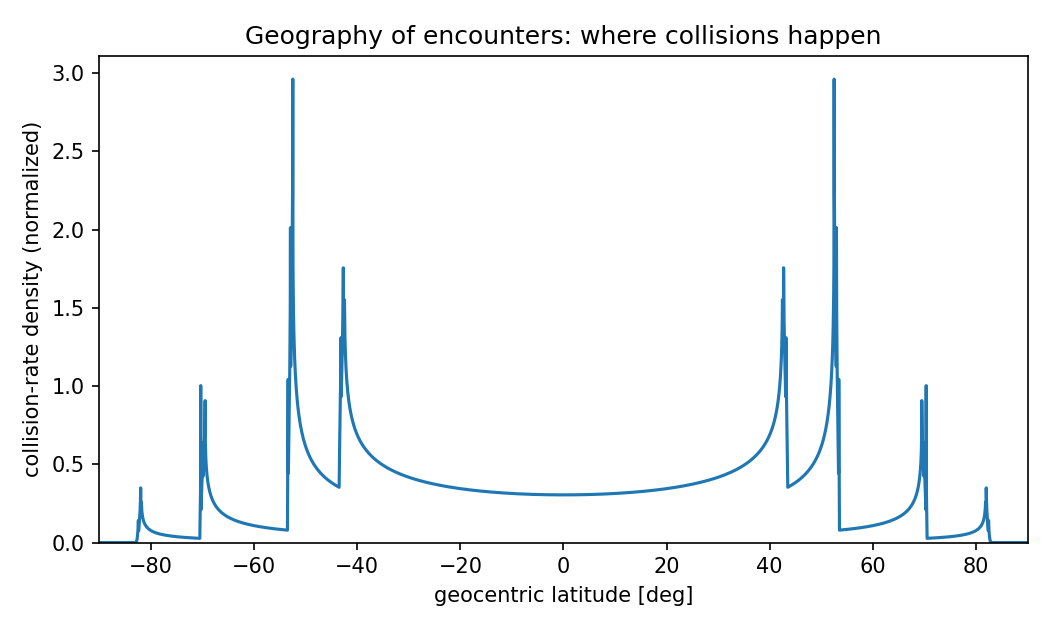
\includegraphics[width=0.70\textwidth]{figures/fig2_rate_latitude.png}
\caption{Normalized collision-rate density versus latitude (geography of
encounters). Encounters cluster at the cap latitudes where plane families cross.}
\label{fig:geo}
\end{figure}

\begin{figure}[h]\centering
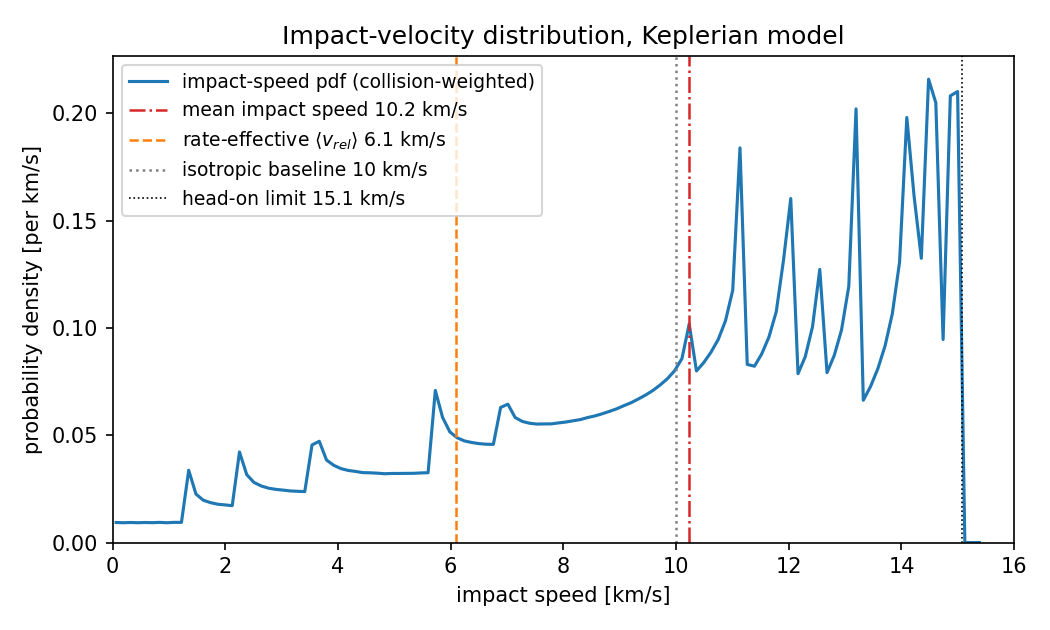
\includegraphics[width=0.70\textwidth]{figures/fig3_velocity_spectrum.png}
\caption{Impact-velocity spectrum of the Keplerian model (collision-weighted).
Cusps correspond to inclination-pair branches; the mass sits at 10--15~km/s.}
\label{fig:spectrum}
\end{figure}

\subsection{Radial concentration}

Compressing the same population into a single 10~km thick shell at 650~km altitude
multiplies the rate by the radial factor ratio
$V/(4\pi r_0^2 w) \approx 30$: $58{,}200$ collisions per year. Spreading in altitude
is worth a factor $\Delta r / w$ in rate, the one geometric lever that does work, with
the caveat that a coordinated single-shell constellation would in practice use phasing
and relative station-keeping that violate the random-element assumption between
same-shell satellites; the figure is the uncoordinated limit.

\section{Monte Carlo validation}

Populations are drawn from the same element distributions and propagated with exact
two-body dynamics (no perturbations, as the analytic model assumes; $J_2$ would only
accelerate the RAAN randomization the analytic model already takes as given).

\textbf{Cube estimator (Liou et al.).} Space is partitioned into cubes of side $h$ at
random epochs and the kinetic rate $\sigma \vrel / h^3$ is accumulated over satellite
pairs found in the same cube, using the true instantaneous velocities. At $N = 2000$
(analytic prediction 1.213 collisions/yr scaled by $(N/80000)^2$), the estimator gives
1.06, 1.13, 1.15 ($\pm 0.02$--$0.03$) at $h = 100, 50, 25$~km, converging from below
toward the analytic value with the expected $O(h)$ bias: by Jensen's inequality the
cube-mean of $n^2$ underestimates $\int n^2$ wherever density varies inside a cell,
and the cap structures have $\sim 60$~km width at $\delta i = 0.5^\circ$.

\textbf{Direct conjunction counting (ground truth).} With $N = 1000$ and an inflated
capture radius $R_c = 5$~km ($\sigma_c = \pi R_c^2$), every close approach is counted
by exact propagation, a radial prefilter (circular orbits cannot approach closer than
$|r_1 - r_2|$), and linearized minimum-distance refinement within 10~s steps. Over 7
simulated days across 4 independent populations: 954 events against
$135.9$/day predicted,
\begin{equation}
\frac{\text{measured}}{\text{analytic}} = 1.003 \pm 0.032 .
\end{equation}
This is a no-kinetic-assumption validation of Eq.~\eqref{eq:rate} at the 3\% level
(Figure~\ref{fig:mc}). Seed-to-seed scatter (107--165 events/day) exceeds Poisson
noise, directly exhibiting the finite-draw fluctuation of criterion (ii).

\begin{figure}[h]\centering
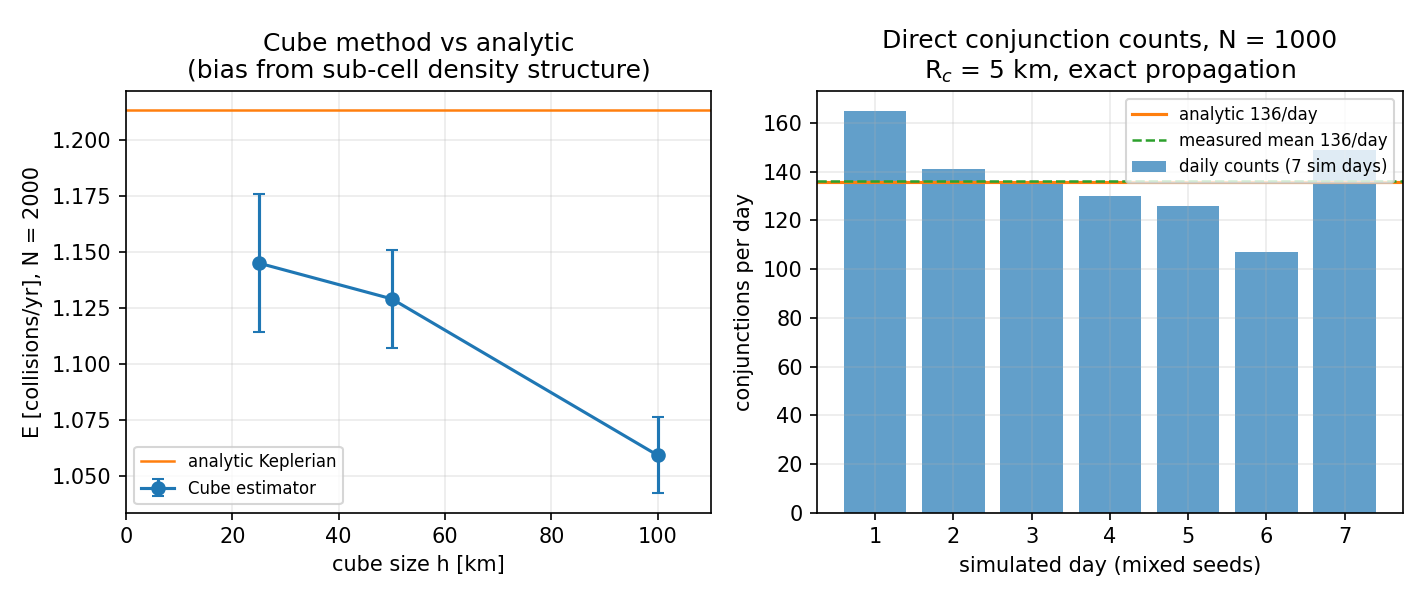
\includegraphics[width=0.95\textwidth]{figures/fig7_mc_validation.png}
\caption{Left: Cube estimator versus cube size, converging to the analytic rate with
the expected resolution bias. Right: direct conjunction counts per simulated day
versus the analytic prediction.}
\label{fig:mc}
\end{figure}

\section{Sensitivity, scaling, and the cascade boundary}

\textbf{Scaling laws.} Per-satellite risk scales as $N \sigma \vrel / V \propto N
r^2 v$; fleet-wide collisions as $N^2 \sigma \vrel / V$. Halving the radiator linear
dimension (quartering $A$) quarters both. Figures~\ref{fig:trade} and the engine
provide the full maps; at $N = 80{,}000$, reaching one natural collision per year
would require $A \approx 0.06\,\mathrm{m}^2$, which no compute payload satisfies:
cross-section alone cannot close the problem either.

\begin{figure}[h]\centering
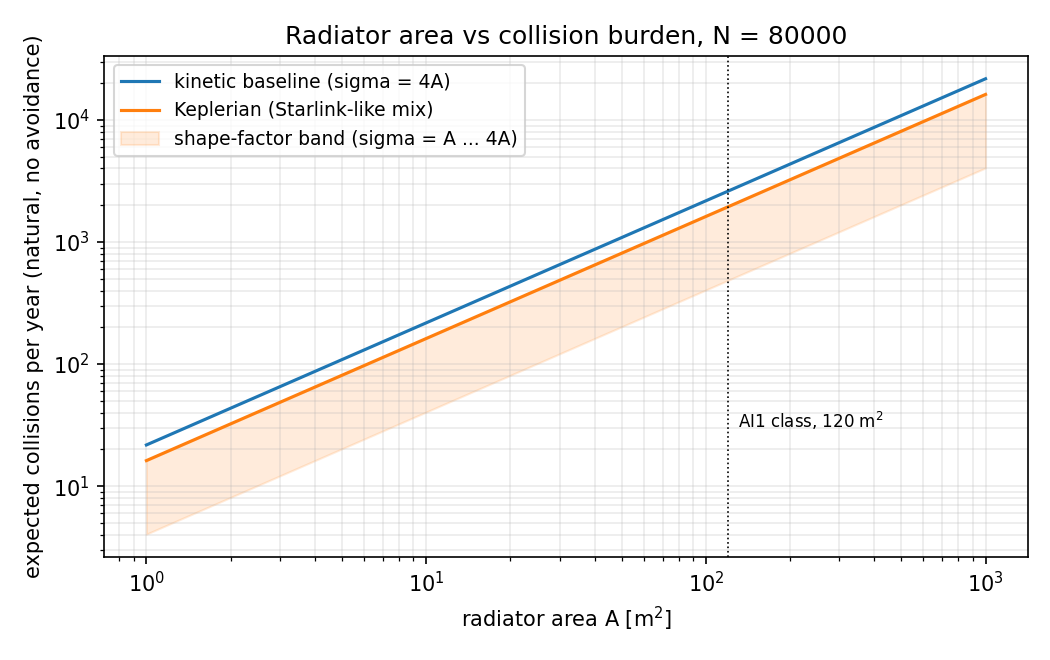
\includegraphics[width=0.70\textwidth]{figures/fig4_radiator_trade.png}
\caption{Radiator area versus natural collision burden for both models, with the
shape-factor band $\sigma = A \ldots 4A$.}
\label{fig:trade}
\end{figure}

\textbf{Natural rate versus residual collisions.} The numbers above are natural
(uncontrolled) rates: they quantify the avoidance \emph{workload}, not the expected
losses. With avoidance failure fraction $f_{\mathrm{fail}}$ applied to the Keplerian
rate of 1941/yr: $f_{\mathrm{fail}} = 10^{-2}$ leaves 19.4 collisions/yr,
$10^{-3}$ leaves 1.9/yr, $10^{-4}$ leaves 0.19/yr. The operational load is set not by
$\sigma$ but by the screening threshold: scaling the rate by $\pi d_{\mathrm{miss}}^2
/ \sigma$, each satellite experiences $\sim 320$ approaches within 1~km per year
($\sim 0.9$ per day), some fraction of which trigger maneuvers. A residual below one
collision per year fleet-wide therefore demands avoidance reliability beyond
$99.95\%$ \emph{including} dead satellites, which is why post-failure disposal
reliability dominates the risk budget in practice.

\textbf{Kessler-cascade boundary.} A first-order branching criterion: one
catastrophic collision creates $F$ lethal fragments with residence time $\tau$;
each hits the constellation at rate $\nbar \sigma_f \vrel$ (avoidance does not apply
to largely untracked debris). The branching number
\begin{equation}
\kappa = F\, \nbar\, \sigma_f\, \vrel\, \tau
\end{equation}
separates self-limiting debris growth ($\kappa < 1$) from runaway ($\kappa > 1$).
With $F = 1000$, $\tau = 25$~yr, $\sigma_f = A$: $\kappa \approx 408$ for the
reference case; $\kappa = 1$ at $N \approx 200$ satellites of this size in this band
(Figure~\ref{fig:cascade}). The reference constellation sits more than two orders of
magnitude beyond the boundary: any catastrophic collision is supercritical, and the
constellation's viability rests entirely on preventing the first ones and on
aggressive post-mission disposal shortening $\tau$. The criterion is deliberately
simple (catastrophic-only collisions, fixed $F$ and $\tau$, band-confined fragments)
and is exposed parametrically in the engine.

\begin{figure}[h]\centering
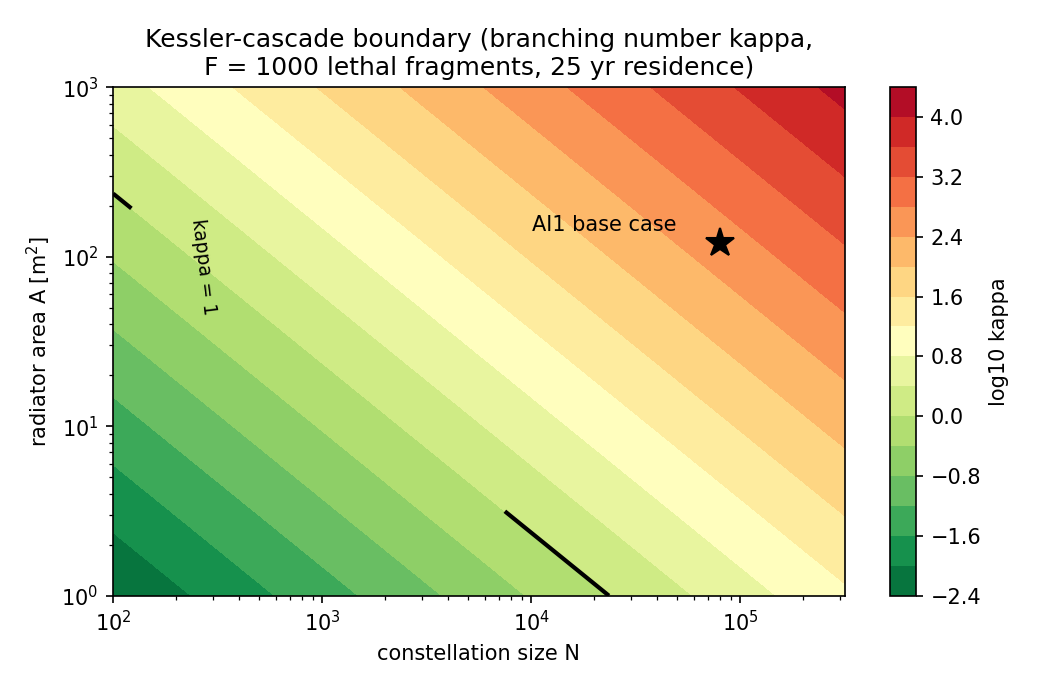
\includegraphics[width=0.70\textwidth]{figures/fig8_cascade_map.png}
\caption{Branching number $\kappa$ in the $(N, A)$ plane; the black contour is
$\kappa = 1$. The reference case lies deep in the supercritical region.}
\label{fig:cascade}
\end{figure}

\section{Implications for design}
\label{sec:implications}

The Keplerian analysis sharpens, and does not soften, the baseline's verdict. The
26\% rate reduction is immaterial against a burden of order $2000$ natural collisions
per year. What the Keplerian model adds is structure with direct design
consequences. First, the radiator trade is quadratic and unforgiving:
collision burden scales with $A$, thermal rejection roughly with $A$, so every unit
of compute-driven heat carries a proportional collision tax that only population or
control can pay. Second, risk is geographically concentrated: conjunction screening
and maneuver capacity should be sized for the cap latitudes of the chosen
inclinations, where both density and crossing geometry stack. Third, the velocity
dichotomy matters for consequence modeling: rates are set by a 6~km/s effective
speed, but the collisions that do occur cluster at 10--15~km/s and are
overwhelmingly catastrophic, feeding the supercritical cascade arithmetic. Fourth,
inclination architecture is a real lever: per-satellite risk varies by $\sim50\%$
across populations, and co-planing reduces crossing terms while radial spreading
buys a factor $\Delta r / w$. Finally, the only quantities that close the problem are
active: avoidance reliability (including dead-satellite disposal) at the
$10^{-3}$--$10^{-4}$ failure level, and debris suppression to pull $\kappa$ toward
unity from above.

\section{Extensions: the integrated systems model}
\label{sec:extensions}

The collision engine has since been embedded in an end-to-end systems model
(the interactive companion at \texttt{megaconstellations.golkar.ai}) that couples
orbit architecture, thermal design, power design, attitude control, and the external
debris environment through one parameter set. This section records the quantitative
results of those extensions; every figure below is generated by the same verified
engine, with the reference scenario of Table~1 unless stated.

\subsection{Sun-synchronous architectures}

Thermal and power designers prefer Sun-synchronous orbits for stable radiator and
array orientation. Locking inclination to altitude through the $J_2$ condition
($i = 97.4^\circ$ at 500~km to $98.5^\circ$ at 800~km, satellites spread evenly
across the band in radially disjoint sub-shells) raises the natural collision rate
to 2689 per year, 38.5\% above the mixed-inclination base case: every near-polar
plane crosses every other at steep angles, and the traffic concentrates at the
polar caps. The orientation convenience carries a collision tax. The harder variant,
clustering every satellite at one local time of the ascending node (all dawn-dusk),
violates the randomized-RAAN assumption of any kinetic model, ours included, and
remains the most important open modeling case for this system class.

\subsection{Thermal coupling: GPU temperature drives the cross-section}

A two-phase pumped-loop model sizes the radiator from the junction temperature:
$T_{\mathrm{rad}} = T_j - \Delta T_{j\to c} - \Delta T_{c\to r}$ and
$A = Q / [2\epsilon\eta\sigma_{SB}(T_{\mathrm{rad}}^4 - T_{\mathrm{sink}}^4)]$,
both faces radiating. For an 80~kW IT node with overhead factor 1.3 (104~kW
rejected), $T_j = 85\,^\circ$C and 28~K of interface drops give
$T_{\mathrm{rad}} = 330$~K and $A = 116.6\,\mathrm{m}^2$, independently consistent
with the 120~$\mathrm{m}^2$ AI1 assumption, at 491~kg of thermal hardware
(6.1~kg per IT~kW). Because the collision rate is linear in $A$ and the radiated
flux scales as $T_{\mathrm{rad}}^4$, junction temperature becomes a collision-risk
lever: running hotter silicon buys quadratically smaller radiators and
proportionally fewer collisions.

\subsection{Power subsystem: the second large area}

PV sizing with eclipse recharge gives, for the same node, $716\,\mathrm{m}^2$ of
array in the worst-case $\beta = 0$ orbit (35~min eclipse, 83~kWh battery,
3810~kg power subsystem) and $429\,\mathrm{m}^2$ in a dawn-dusk orbit
(no battery, 2536~kg). The dawn-dusk specific area, $5.37\,\mathrm{m}^2$ per IT~kW,
independently reproduces Turyshev's published anchor of $5.64\,\mathrm{m}^2$/kW
within 5\%. The consequence for collision risk is severe: the PV array, not the
radiator, is the largest deployed surface. Counting it in the collision
cross-section ($A = 120 + 716 = 836\,\mathrm{m}^2$) multiplies the natural rate by
6.96, to roughly 13{,}500 collisions per year. The radiator tax of the original
analysis is really a deployed-area tax, about three times larger than charged.

\subsection{Attitude control feasibility}

The deployed area also sets the control problem. For the two-wing 33~m
configuration the inertia asymmetry is $\Delta I \approx 40{,}500$~kg\,m$^2$
(maximum axis $42{,}200$~kg\,m$^2$, about half of Hubble's $87{,}000$, and Hubble
flies on reaction wheels). Gravity gradient dominates the disturbance budget:
12.2~mN\,m at a $5^\circ$ sustained offset, against 0.87 (solar pressure), 0.17
(magnetic, 5~A\,m$^2$ residual) and 0.07~mN\,m (aerodynamic, feathered panels).
The cyclic momentum load is 26~N\,m\,s per orbit with margin, served by a standard
four-wheel pyramid (57~kg suite with magnetorquer desaturation at 107~A\,m$^2$)
with a torque-authority margin of order $7\times$ over the peak disturbance. The
real costs of the large structure are agility (a 90$^\circ$ slew takes tens of
minutes, irrelevant for sun/nadir-fixed operation) and controller bandwidth below
the flexible modes of 15~m wings, which this screening level does not model. At
worst-case $45^\circ$ gravity-gradient attitudes the requirement reaches
134~N\,m\,s, the top of the wheel class, and control-moment gyros become
preferable. Configuration is a strong lever: a compact z-fold radiator stack cuts
the momentum requirement to 6.8~N\,m\,s.

\subsection{External debris: the risk channel avoidance cannot touch}

A screening flux layer (hits $= N A_{\mathrm{eff}}\, n\, v_{\mathrm{rel}}$, with an
altitude profile calibrated to public ORDEM~3.1 / MASTER-8 / ESA figures and an
explicit uncertainty scale) adds the environment the fleet does not control. At
the band-average densities ($6.4\times10^{-8}$ and $1.8\times10^{-6}$~km$^{-3}$
for $>$10~cm and $>$1~cm objects), the reference fleet sustains about 780
trackable-object encounters per year, which join the avoidance workload, and about
5500 lethal non-trackable (1--10~cm) impacts per year, 0.068 per satellite-year,
which no avoidance can prevent. With 30\% of the satellite area mission-critical,
that is roughly 1640 expected losses per year, dwarfing the avoidance-residual
budget. The two risk channels are structurally decoupled: $f_{\mathrm{fail}}$
suppresses satellite-satellite losses, while only damage tolerance, shielding and
segmentation address the non-trackable flux, and only fragmentation suppression
and disposal address $\kappa$. The lethal non-trackable population anchor here is
deliberately tied to ESA object counts and sits at the upper edge of the indicative
band of the external review; a bankable assessment requires native ORDEM/MASTER
runs with the real geometry.

\subsection{Benchmark validation}

Two independent published analyses now bracket this work. An external
due-diligence reconstruction (10~June 2026) rebuilt the collision model from the
governing integral and reproduces eleven quantities of this report to three or
more digits (rates, scalings, thresholds, $\kappa$, screening load). Turyshev
(arXiv:2604.27197) provides the independent power/thermal anchor, reproduced here
on PV specific area within 5\%; his economics treat collisions only as an
aggregated hazard rate, and this model supplies the fleet-level physics behind
that term, including the correlated cascade risk an independent-hazard framework
cannot represent. The interactive companion currently carries a live validation
table and chart against the Turyshev anchors.

\section{Key conclusions}

Eight results summarize the study. (1)~The convergence hypothesis holds in refined form:
randomized Keplerian dynamics is exactly a kinetic theory with the structured density
field \eqref{eq:density} and the discrete velocity spectrum \eqref{eq:vrelbranches};
the isotropic Maxwellian closure is the one casualty, overestimating the reference rate
by 34\% while misrepresenting the velocity spectrum entirely. (2)~The reference
constellation (80{,}000 satellites, $\sigma = 4A = 480\,\mathrm{m}^2$, 500--800~km)
sustains a natural rate of 1941 collisions per year, validated to $0.3\% \pm 3.2\%$
against direct conjunction counting; per-satellite risk is 4.2--6.2\% per year depending
on inclination. (3)~No shell geometry brings the natural rate to acceptable levels; the
inversion requires filling space beyond GEO for one collision per year. The only
geometric lever that works is radial spreading, worth the ratio of band thickness to
shell width. (4)~Collision \emph{rates} are governed by an effective 6.1~km/s relative
speed, but the collisions that occur cluster at 10--15~km/s and are catastrophic; with
$F = 1000$ lethal fragments and 25-year residence, the cascade branching number is
$\kappa \approx 400$, so the constellation's viability rests entirely on preventing
first collisions. (5)~The collision burden scales as $N^2 \sigma$: radiator area is a
linear collision tax on compute capacity, and avoidance reliability of $10^{-3}$
failure or better, including failed satellites, is the gating requirement.
(6)~The deployed-area tax is roughly three times larger than the radiator-only
accounting: the PV array (716~$\mathrm{m}^2$ per 80~kW node in eclipse-prone
orbits, 429~$\mathrm{m}^2$ dawn-dusk) dominates the cross-section, and counting it
multiplies the natural rate by 7, to roughly 13{,}500 per year. (7)~The
thermally and electrically preferred Sun-synchronous architecture raises the
collision rate 38.5\% over the mixed base case; orbit convenience and collision
risk pull in opposite directions. (8)~External lethal non-trackable debris adds a
loss channel of order $10^3$ per fleet-year that no avoidance reliability can
reduce; damage tolerance and segmentation therefore belong in the same gating set
as avoidance and disposal. Attitude control, by contrast, is not a blocker:
despite 33~m spans the inertia is Hubble-class and standard reaction-wheel suites
carry order-$7\times$ torque margins.

\section{Validity of approximations}

\begin{table}[h]\centering\small
\begin{tabular}{lll}
\toprule
Assumption & Where used & Validity \\
\midrule
Dilute gas, Poisson & both models & $\lambda/\Delta r \sim 10^{7}$, $\nu T \ll 1$: excellent \\
Thin shell $V \approx 4\pi\Rbar^2\Delta r$ & baseline checks & error $0.1\%$ for 300 km band \\
Isotropy + Maxwellian & baseline only & wrong in structure; net rate error $+34\%$ \\
Circular orbits & Keplerian model & $e \lesssim 10^{-3}$ shifts densities by km: negligible on rate \\
$\vorb$ at $\Rbar$ in $J_{jk}$ & Keplerian model & $<2\%$ across band \\
No perturbations & both & $J_2$ only randomizes RAAN faster: helps assumptions \\
Element randomization & Keplerian model & exact for ensemble; finite-draw scatter per criterion (ii) \\
Gravitational focusing neglected & both & corrections $O(10^{-14})$ \\
Shape factor $\sigma = 4A$ & both & physical band $\sigma = (1\ldots4)A$, all rates linear in $\sigma$ \\
\bottomrule
\end{tabular}
\caption{Approximation register.}
\end{table}

\section*{Deliverables and reproduction}

\texttt{collision\_models.py} implements both models with inputs and derived
quantities strictly separated (Inputs dataclass: $N$, $A$, shape factor, band,
radial profile, inclination mix and dispersion, $\vrel^{\mathrm{iso}}$,
$f_{\mathrm{fail}}$, $T$, cascade parameters; outputs: rates, per-satellite
probabilities, mean free path, expected collisions, model ratio and its
decomposition, velocity and latitude distributions, cascade boundary).
\texttt{montecarlo\_validation.py} contains the Cube estimator and the direct
conjunction counter. \texttt{analysis\_figures.py} regenerates every figure and
\texttt{results\_summary.json}, from which all numbers in this report are taken.
Running \texttt{python3 collision\_models.py} prints the anchor checks
(2608 collisions/yr baseline). The formulation is modular: all engine functions are
closed-form or single quadratures, with no hidden state. The interactive systems
model built on this engine, including the thermal, power, attitude-control and
external-debris layers of Section~\ref{sec:extensions} and the live benchmark
validation, is deployed at \texttt{https://megaconstellations.golkar.ai} with
source at \texttt{github.com/agolkar/orbit-collisions}.

\section*{References}

Kessler, D.~J., Cour-Palais, B.~G. (1978). Collision frequency of artificial
satellites: the creation of a debris belt. \emph{JGR} 83(A6), 2637--2646.
\quad
Kessler, D.~J. (1981). Derivation of the collision probability between orbiting
objects: the lifetimes of Jupiter's outer moons. \emph{Icarus} 48, 39--48.
\quad
\"Opik, E.~J. (1951). Collision probabilities with the planets. \emph{Proc.~R.
Irish Acad.} 54A, 165--199.
\quad
Wetherill, G.~W. (1967). Collisions in the asteroid belt. \emph{JGR} 72, 2429--2444.
\quad
Liou, J.-C., Hall, D.~T., Krisko, P.~H., Opiela, J.~N. (2004). LEGEND: a
three-dimensional LEO-to-GEO debris evolutionary model. \emph{Adv.~Space Res.}
34, 981--986.

\end{document}
